\documentclass[a4paper,12pt]{article}

\usepackage{Packages}
\usepackage{breqn}
\usepackage{amsmath}
\long\def\/*#1*/{}

\begin{document}
\begin{titlepage}

\begin{center}

% Upper part of the page. The '~' is needed because \\
% only works if a paragraph has started.

\includegraphics[width=0.6\textwidth]{./Figures/TUe}~\\[2cm]


%\vspace*{10cm}

% Title
\HRule \\[0.4cm]
{ \huge \bfseries 2IMM20 - Foundations of datamining\\[0.3cm] }
\HRule \\[1.5cm]
\textbf{Assignment 2}


% Author and supervisor

\vfill

\begin{table}[h]
\begin{tabular}{ll}
\textbf{Students:} & \\
Joris van der Heijden & (0937329)\\
Bram van der Pol & (0780042)\\

\\
\textbf{Email addresseses:} & \\
j.j.m.v.d.heijden@student.tue.nl \\
a.f.v.d.pol@student.tue.nl \\
\\
\textbf{Supervisors:} &\\
Dr.ir. Joaquin Vanschoren
\\

%\textbf{Supervisors:} & \\
%Dr. M.Holenderski \\
\end{tabular}
\end{table}



% Bottom of the page
\large
{ Eindhoven, \today}

\end{center}


\end{titlepage}
 %included in part 1
\tableofcontents %included in part 1

\newpage	
\section{Backstepping}
\subsection{Exercise 1} %Exercise 1

The dynamics in $x$ variables is obtained by rewriting the given error variables and substituting these in the original system dynamics equations. The resulting dynamics in $x$ coordinates is then given by $\dot{x} = f(x) + g(x)u$ where:

\begin{align}
f=
\begin{bmatrix}
 -\frac{1}{2}\sigma \,x_{1}\,\left({\left(x_{2}+1\right)}^2+{x_{1}}^2-1\right) \\
\frac{3\,x_{2}}{2}+x_{3}-\frac{{\left(x_{2}+1\right)}^3}{2}-3{x_{1}}^2\,\left(\,x_{2}+1\right)+\frac{1}{2}\\
0
\end{bmatrix} \quad and, \quad
g=
\begin{bmatrix}
0\\
0\\
1
\end{bmatrix}
\label{eq:Xsystem}
 \end{align}

\subsection{Exercise 2} %Exercise 2
The stability of the $x_1$ subsystem (with $x_2=0$) is checked by means of a Lyapunov function. The proposed Lyapunov function and its time derivative is given by: \ref{eq:LyapunovQ2a} and \ref{eq:LyapunovQ2}

\begin{flalign}
V_1 &=\frac{1}{2}x_1^2 \label{eq:LyapunovQ2a} \\
\dot{V}_1&=x_1\dot{x_1}=-\frac{1}{2}\sigma \,x_{1}\,\left({\left(x_2+1\right)}^2+{x_{1}}^2-1\right) \label{eq:LyapunovQ2} \\
\nonumber &=-\frac{1}{2}\sigma \,x_{1}\,\left(1+{x_{1}}^2-1\right)= -\frac{1}{2}\sigma x_1^4
\end{flalign}

The function \ref{eq:LyapunovQ2} is negative definite for all $x_1$ values and therefore the controller ($x_2 = 0$) stabilizes the subsystem $x_1$.

\subsection{Exercise 3} %Exercise 3
First we introduce a coordinate transformation by using the virtual control stated in question 2 ($x_2^v=\alpha(x_1)= 0$): 
\begin{flalign}
z_1&=x_1\\
z_2&=x_2 - \alpha(x_1) = x_2
\end{flalign}
Therefore the reverse transformation is given by:
\begin{flalign}
x_1&=z_1 \label{eq:x1z1}\\
x_2&=z_2 \label{eq:x2z2}
\end{flalign}

The time derivative are calculated for this coordinate transformation:
\begin{flalign}
\dot{z_1}&=\dot{x_1}= -\frac{1}{2}\sigma \,x_{1}\,\left({\left(x_{2}+1\right)}^2+{x_{1}}^2-1\right) \label{vd1}\\
\dot{z_2}&=\dot{x_2} = \frac{3\,x_{2}}{2}+x_{3}-\frac{{\left(x_{2}+1\right)}^3}{2}-3{x_{1}}^2\,\left(\,x_{2}+1\right)+\frac{1}{2} \label{vd2}
\end{flalign}
By using the backward coordinate transformation (\ref{eq:x1z1} and \ref{eq:x2z2}) the z derivatives in $z$ variables is given by:

\begin{flalign}
\dot{z_1}&=\dot{z_1}= -\frac{1}{2}\sigma \,z_{1}\,\left({\left(z_{2}+1\right)}^2+{z_{1}}^2-1\right) \label{vd1_z}\\
\dot{z_2}&=\dot{z_2} = \frac{3\,z_{2}}{2}+x_{3}-\frac{{\left(z_{2}+1\right)}^3}{2}-3{z_{1}}^2\,\left(\,z_{2}+1\right)+\frac{1}{2} \label{vd2_z}
\end{flalign}

The variable $x_3$ appears in the equations, which is the virtual control input which is needed. To guarantee stability in the z domain the Lyapunov function $V_2$ is introduced: 

\begin{align}
V_2=V_1(z_1)+\frac{1}{2}z_2^2\\
\dot{V_2}=z_1\dot{z_1}+z_2\dot{z_2}
\label{eq:V2dsimple}
\end{align}

The variables $\dot{z_1}$ and $\dot{z_2}$ from equation \ref{vd1_z} and \ref{vd2_z} are substituted in equation \ref{eq:V2dsimple}:
\begin{align}
\dot{V}_2 = z_{2}\,\left(x_{3}+\frac{3\,z_{2}}{2}-\frac{{\left(z_{2}+1\right)}^3}{2}-{z_{1}}^2\,\left(3\,z_{2}+3\right)+\frac{1}{2}\right)-\frac{\sigma \,{z_{1}}^2\,\left({\left(z_{2}+1\right)}^2+{z_{1}}^2-1\right)}{2}
\label{eq:V2d}
\end{align}
The goal is to choose a $x_3^v$ that replaces $x_3$ in $\dot{V}_2$ which ensures that the Lyapunov function becomes negative definite, which can be achieved by stating that: 
\begin{align}
\dot{V_2}= -c_1z_1^2-c_2z_2^2 \\
\end{align}
Here: $c_1,c_2$ are positive and are used to place the poles in exercise 12. The resulting $x_3^v$ controller is given by \ref{eq:x3v}. 
\begin{equation}
x_3^v = \frac{6\,{z_{1}}^2\,{z_{2}}^2-2\,c_{1}\,{z_{1}}^2-2\,c_{2}\,{z_{2}}^2+\sigma \,{z_{1}}^4+6\,{z_{1}}^2\,z_{2}+3\,{z_{2}}^3+{z_{2}}^4+2\,\sigma \,{z_{1}}^2\,z_{2}+\sigma \,{z_{1}}^2\,{z_{2}}^2}{2\,z_{2}}
\label{eq:x3v}
\end{equation}

We choose to cancel all terms despite some are already negative definite because this simplifies the next Lyapunov function ($V_3$). 

\subsection{Exercise 4} %Exercise 4
In order to obtain the final controller $u$ the coordinate transformation is expanded with:
\begin{flalign}
z_3&=x_3 - x_3^v(x)
\label{eq:z3}
\end{flalign}
And the reverse coordinate transformation:
\begin{flalign}
x_3&=z_3 + x_3^v(z)
\label{eq:z3_z}
\end{flalign}

the time derivative of $z_3$ is given by:
\begin{flalign}
\dot{z}_3  &= \dot{x}_3 - \frac{\partial x_3^v}{\partial z} \dot{z}
\label{eq:z3d}
\end{flalign}

To find a solution for the control input $u$ we use the Lyapunov function: 
\begin{flalign}
V_3&=V_2+\frac{1}{2}z_3^2
\label{eq:V3}
\end{flalign}
The time derivative of $V_3$ is given by:
\begin{flalign}
\dot{V_3}&=z_1\dot{z_1}+z_2\dot{z_2}+z_3\dot{z_3}
\end{flalign}

The input can be solved using this Lyaponov function, this function must be negative definite in $z_3$ domain. This is achieved by solving:

\begin{align}
\dot{V}_3=z_1\dot{z_1}+z_2\dot{z_2}+z_3 \dot{z_3} = -c_3z_3^2
\label{eq:V3d}
\end{align}
for the control input $u$. Variable $x_3$ is substituted by using the reverse coordinate transformation form $z$ to $x$. The solution is given in \ref{eq:u_z} in the appendix.

\subsection{Exercise 5} %Exercise 5
The derivative of the Lyapunov function is given by:
\begin{align}
\dot{V}_2 = 2c_1x_1\dot{x_1}+\sigma x_2\dot{x_2}
\end{align}
With the use of the proposed equation for $x_3$ the equation is rewritten to:
\begin{align}
\dot{V}_2(x_1,x_2)=-\frac{1}{2}\sigma(6x_1^2x_2^2+2c_1x_2^2+2c_1x_1^4+x_2^2+4c_1x_1^2x_2+2c_1x_1^2x_2^2)
\end{align}
The ($x_1,x_2$)-subsystem is stable if $\dot{V}_2$ is negative definite for all $x_1$ and $x_2$. In the equation above all the terms without $c_1$ will not cause the equation to become positive. Therefore for the rest of this exercise these terms will be not be taken into account. The terms of $\dot{V}_2$ with only $c_1$ term is given by:
\begin{align}
\dot{V}_{2}(x_1,x_2)=-\frac{1}{2}\sigma(2c_1x_2^2+2c_1x_1^4+4c_1x_1^2x_2+2c_1x_1^2x_2^2)
\end{align}
which can be rewritten to:
\begin{align}
\dot{V}_{2}(x_1,x_2)=-\sigma c_1((x_1^2+x_2)^2+x_1^2x_2^2)
\end{align}
Which is negative definite for all $x_1$ and $x_2$ due to the squared term, resulting in the proof that the proposed virtual input for $x_3$ and the given Lyapunov function will result in a stable $(x_1 , x_2)$-subsystem.

\subsection{Exercise 6} %Exercise 6
First, the coordinate transformation is performed as shown in Exercise 4, equations \ref{eq:z3} and \ref{eq:z3d}. The time derivative of the proposed virtual input is given by \ref{eq:V3d6} which can be found in the appendix. The same Lyapunov function is used as in question 4 (equation \ref{eq:V3}) to guarantee stability. The derivative is given by equation \ref{eq:V3dsimple}, the complete version is equation \ref{eq:V3d6} which can be found in the appendix. This function is forced to be negative definite to ensure stability. Here variable $c_2$ and $c_3$ are introduced which are used in exercise 12.
\begin{equation}
\dot{V}_3 = \dot{V}_2 + z_3\dot{z_3} = -c_2z_2^2-c_3z_3^2
\label{eq:V3dsimple}
\end{equation}

When this equation is solved for control input $u$, equation \ref{eq:uz6} is found.

\newpage
\section{Feedback Linearisation}
\subsection{Exercise 7}
The conditions for feedback linearizability are given in the box below, where $n$ denotes the state dimension. For the system that is considered, n = 3.

\noindent\makebox[\linewidth]{\rule{\textwidth}{0.4pt}}
\begin{align}\label{conditions}
&D_i=span(g_1(x),...,g_m(x),...,ad^i_fg_1(x),...,ad^i_fg_m(x)),\textrm{ for i = $0,1,2,3$}\\ \nonumber
&\textrm{1. Where each distribution $D_i$ has constant dimension}\\ \nonumber
&\textrm{2. $D_{n-1}$ has dimension 3}\\ \nonumber
&\textrm{3. Each distrubution $D_i$ is involutive for $i=0,1,2,3$}
\end{align}
\noindent\makebox[\linewidth]{\rule{\textwidth}{0.4pt}}

The conditions 1,2 and 3 from \ref{conditions} are checked for $D_0$:
\begin{align}\label{D0}
D_0=span\left\{\begin{pmatrix} 0\\0\\1  \end{pmatrix}\right\}
\end{align}
Equation \ref{D0} shows that the distribution has a constant dimension 1. Furthermore this vector is involutive because it is constant and has dimension 1. Since the rank of $D_0$ does not equal 3, the next distribution ( $D_1$) is checked:
\begin{align}\label{D1}
D_1=span\left\{\begin{pmatrix} 0 \\ 0 \\ 1 \end{pmatrix} , \begin{pmatrix}
0 \\ -1 \\ 0\end{pmatrix} \right\}
\end{align}

The distribution $D_1$ has a constant dimension. The involutiveness is checked by checking if the Lie brackets of $D_1$ are spanned by $D_1$:
\begin{align}
[g_1,g_2] = \frac{\partial{g_2}}{\partial{x}}g_1-\frac{\partial{g_1}}{\partial{x}}g_2= [0\ 0\ 0\ 0]^T\in D_0\\ \nonumber
[g_2,g_1] = \frac{\partial{g_1}}{\partial{x}}g_2-\frac{\partial{g_2}}{\partial{x}}g_1
 = [0\ 0\ 0\ 0]^T\in D_0\\ \nonumber
\end{align}

Since the rank of $D_1$ does not equal 3  the next distribution ($D_2$) is checked on the 3 conditions (\ref{conditions}). 

\begin{align}\label{D2}
D_2=span\left\{
\begin{pmatrix} 0 \\ 0 \\ 1 \end{pmatrix} 
, \begin{pmatrix} 0 \\ -1 \\ 0\end{pmatrix}
, \begin{pmatrix} -\frac{\sigma \,x_{1}\,\left(2\,x_{2}+2\right)}{2} \\ \frac{3}{2}-3\,{x_{1}}^2-\frac{3\,{\left(x_{2}+1\right)}^2}{2} \\ 0 \end{pmatrix} 
\right\}
\end{align}
This distribution has a constant dimension if: ($x_1 \neq 0 \wedge x_2\neq-1$). Furthermore $D_2$ is involutive since the rank of the distribution equals the dimension. Thus every Lie bracket must be spanned $D_2$.  Concluding that the system is feedback linearizable if: ($x_1 \neq 0 \wedge x_2\neq-1$).

\subsection{Exercise 8}
To determine the relative degree we use the definition. If in \ref{eq:Lie8.1} for all x the relative degree is $k$. 
\begin{align}
L_gL_f^{k-1}h(x)\neq 0
\label{eq:Lie8.1}
\end{align}

Now we compute the Lie derivatives:  
\begin{align}
L_gh(x)=0 \\
L_gL_fh(x)=1
\label{eq:Lie8}
\end{align}

Therefore the relative degree is 2. Because the value of equation \ref{eq:Lie8} does not dependent on $\textbf{x}$, the relative degree is globally defined.

\subsection{Exercise 9}
We apply the regular state feedback: 
\begin{align} 
u=\left( L_gL_fh(x)\right)^{-1}\left(-L_f^2h(x)+v\right)
\label{eq:standardu}
\end{align}

\begin{dmath}
u = v-L_f^2h(x)
\label{eq:u9}
\end{dmath}

Equation \ref{eq:standardu} is rewritten to: 
\begin{align}
u=\alpha(x)+\beta(x)v
\end{align} 
Therefore:
\begin{dmath}
\alpha(x) =  \left(\frac{3\,{\left(x_{2}+1\right)}^2}{2}+3\,{x_{1}}^2-\frac{3}{2}\right)\,\left(\frac{3\,x_{2}}{2}+x_{3}-\frac{{\left(x_{2}+1\right)}^3}{2}-{x_{1}}^2\,\left(3\,x_{2}+3\right)+\frac{1}{2}\right)-\sigma \,{x_{1}}^2\,\left(3\,x_{2}+3\right)\,\left({\left(x_{2}+1\right)}^2+{x_{1}}^2-1\right)
\end{dmath}

\begin{equation}
\beta(x) = 1
\end{equation}

Using this control feedback equation yields: $\ddot{x_2}=v$. Therefore the system is feedback linearised. 

\subsection{Exercise 10}
Using the coordinate transformation definition:
\begin{align}
\textbf{z} = \Phi(x)=\begin{bmatrix} h(x)\\L_fh(x) \\ \eta \end{bmatrix}
\end{align}

Using the results from the previous exercise:
\begin{align}
\Phi(x)=\begin{bmatrix} x_2\\ \frac{3\,x_{2}}{2}+x_{3}-\frac{{\left(x_{2}+1\right)}^3}{2}-3{x_{1}}^2\,\left(\,x_{2}+1\right)+\frac{1}{2}\\ \eta \end{bmatrix}\\
\Phi^{-1}(z)=\begin{bmatrix}
z_3 \\
z_1 \\
\frac{1}{2}z_1^3+\frac{3}{2}z_1^2+3z_1z_3^2+3z_3^2+z_2
\end{bmatrix}
\end{align}

$\eta=x_1$ is chosen because no algebraic constraints are needed for this choice of $\Phi(x)$. To verify if $\Phi$ and $\Phi^{-1}$ are globally defined the determinant of these matrices is calculated and checked if these are non-zero. This is the case and therefore these state transformations are globally defined. Now the dynamics in $z$ coordinates becomes: 

\begin{align}
\dot{{\bf z}}=\begin{bmatrix} z_2 \\ v \\-\frac{1}{2}\sigma z_3 ((z_1+1)^2+z_3^2-1)
\end{bmatrix}
\label{eq:zd}
\end{align}

\subsection{Exercise 11}
The definition of the zero dynamics is that the reference output is zero ($y_d=x_2=z_1=0$). This also implies that $\dot{y}_d=z_2=0$. This definition is substituted in \ref{eq:zd}. Giving the following system:

\begin{align}
\dot{{\bf z}}=\begin{bmatrix} 0 \\ v \\-\frac{1}{2}\sigma z_3^3
\end{bmatrix}
\label{eq:zd_zero}
\end{align}


In equation \ref{eq:zd_zero} the controller $v$ can be chosen as a PD-controller to stabilizes the system, using the equation:
\begin{align}
\ddot{e}+a_1\dot{e}+a_0e=0
\end{align}
With:
\begin{align}
e = y = x_2 = z_1\\
\dot{e} = \dot{y} = \dot{z_1}=z_2\\
\ddot{e} = \dot{z_2} = v
\end{align}
Therefore:
\begin{align}
v=-a_1z_2-a_0z_1
\label{controller v}
\end{align}

Substituting \ref{controller v} in equation \ref{eq:zd_zero} gives the system:

\begin{align}
\dot{{\bf z}}=\begin{bmatrix} 0 \\ 0 \\-\frac{1}{2}\sigma z_3^3
\end{bmatrix}
\label{eq:zd_zero_PD}
\end{align}

Now the Lyapunov function $V_{3_2}=\frac{1}{2}z_3^2$ is used to show stability for the $z$ system. This Lyapunov function is only a function of $z_3$ because $\dot{z_1}=0$ and $\dot{z_2}=0$. 
\begin{align}
\dot{V}_{3_2}=\dot{z_3}z_3=-\frac{1}{2}\sigma z_3^4
\label{V3d2}
\end{align}

Since equation \ref{V3d2} is negative definite, this system is globally stable. 

\section{Simulation based controller comparison}
\subsection{Exercise 12}
The systems are linearized around the equilibrium point $(x_1=0,x_2=0,x_3=0)$. Unfortunately were unable to place the poles of the controlled closed loop systems, because the linearized system matrix $A$ had a rank of 2 instead of 3 for both the controllers that are designed in exercise 4 and 6.This causes that it is hard to compare the controllers with each other. However to make a comparison all the gains $(c1,c2,c3)$ and $(a_0,a_1)$ are set to $1$. The resulting response of the system is given in Figure \ref{fig:controllers1}. The initial condition are set to $x_0 = [0.5, 0.5, 10]$ because the performance became clearly visible for these initial conditions.

\begin{figure}[H]
\begin{center}
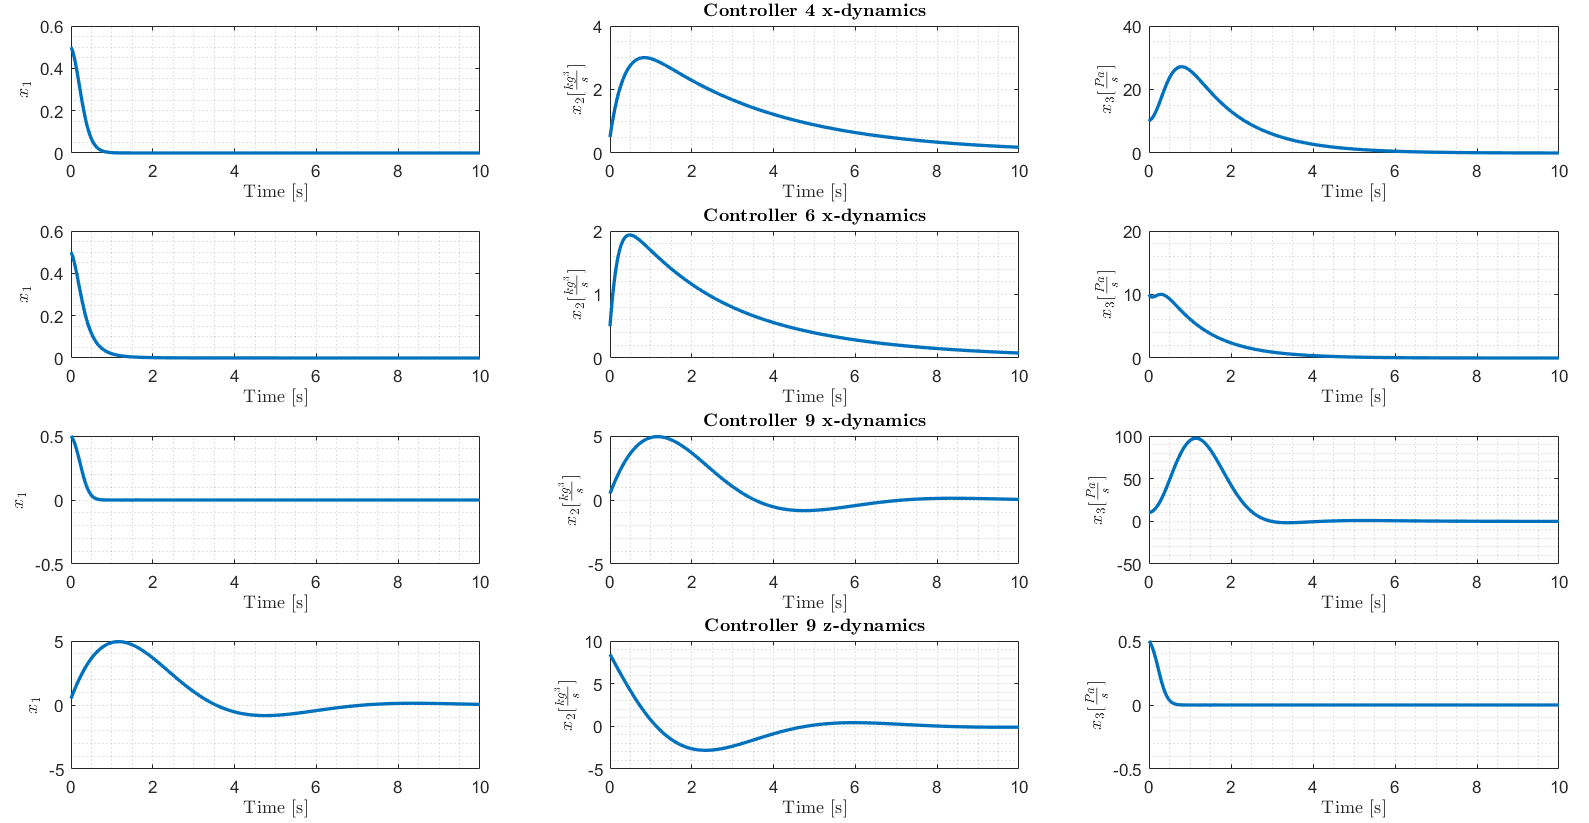
\includegraphics[width= \textwidth]{Figures/controllers.png}
\caption{Response of the system for the three different controllers with initial conditions $x_0 = [0.5, 0.5, 10]$ and $(c1,c2,c3)$ and $(a_0,a_1)$ are set to $1$}
\label{fig:controllers1}
\end{center}
\end{figure}

This figure shows that controller 6 has the best performance in terms of overshoot. The settling time however is the lowest for controller 9, especially for the $x_2$ variable. We discovered that by tuning the parameters $a_0$ and $a_1$ the overshoot and settling time can drastically be reduced. Changing the parameters $c_1,c_2,c_3$ did not show an improvement of the same scale. 

\subsection{Exercise 13}
Since in the system dynamics $\sigma$ is only present in $\dot{x}_1$ the response for $x_1$ is investigated. When $\sigma$  is increased to 2 the settling time clearly decreases for controllers 4 and 6 as can be seen in Figures \ref{fig:sigma1} and \ref{fig:sigma2}. However this decrease in settling time does not hold for controller 9. 


\begin{figure}[H]
\centering
\begin{minipage}{.5\textwidth}
  \centering
  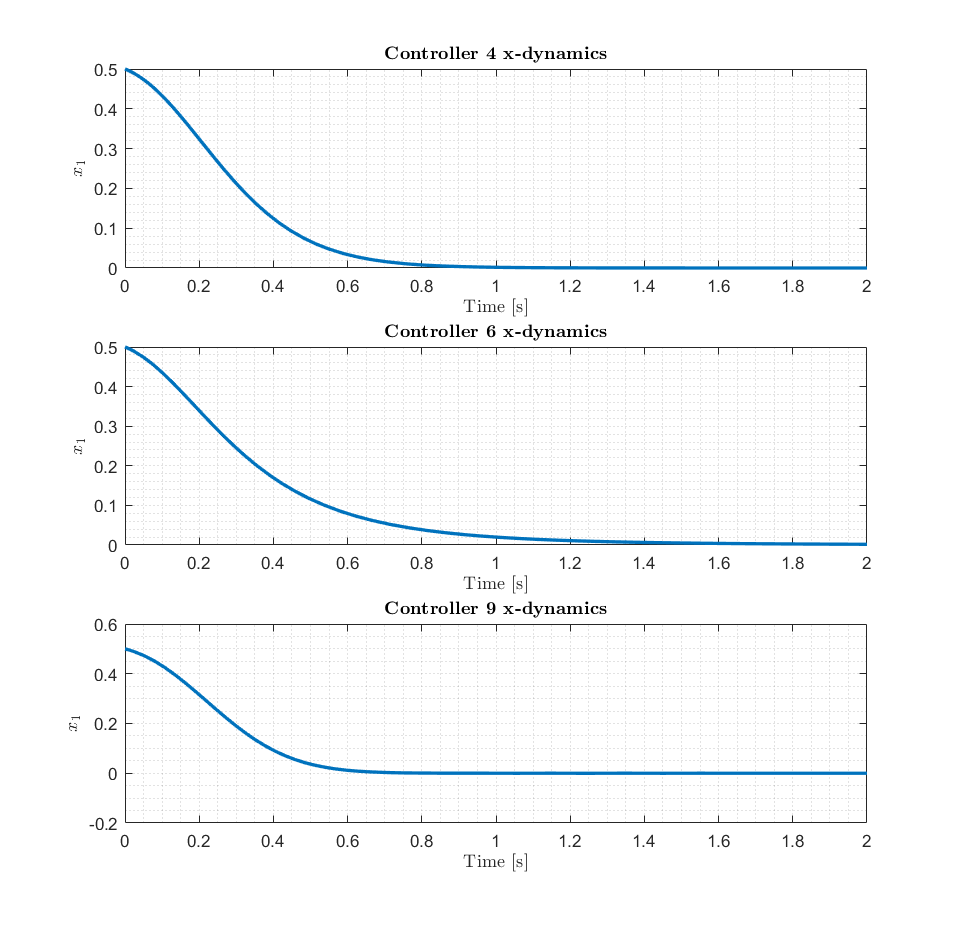
\includegraphics[width=\linewidth]{Figures/sigma_1.png}
  \caption{Response for $\sigma = 1$}
  \label{fig:sigma1}
\end{minipage}%
\begin{minipage}{.5\textwidth}
  \centering
 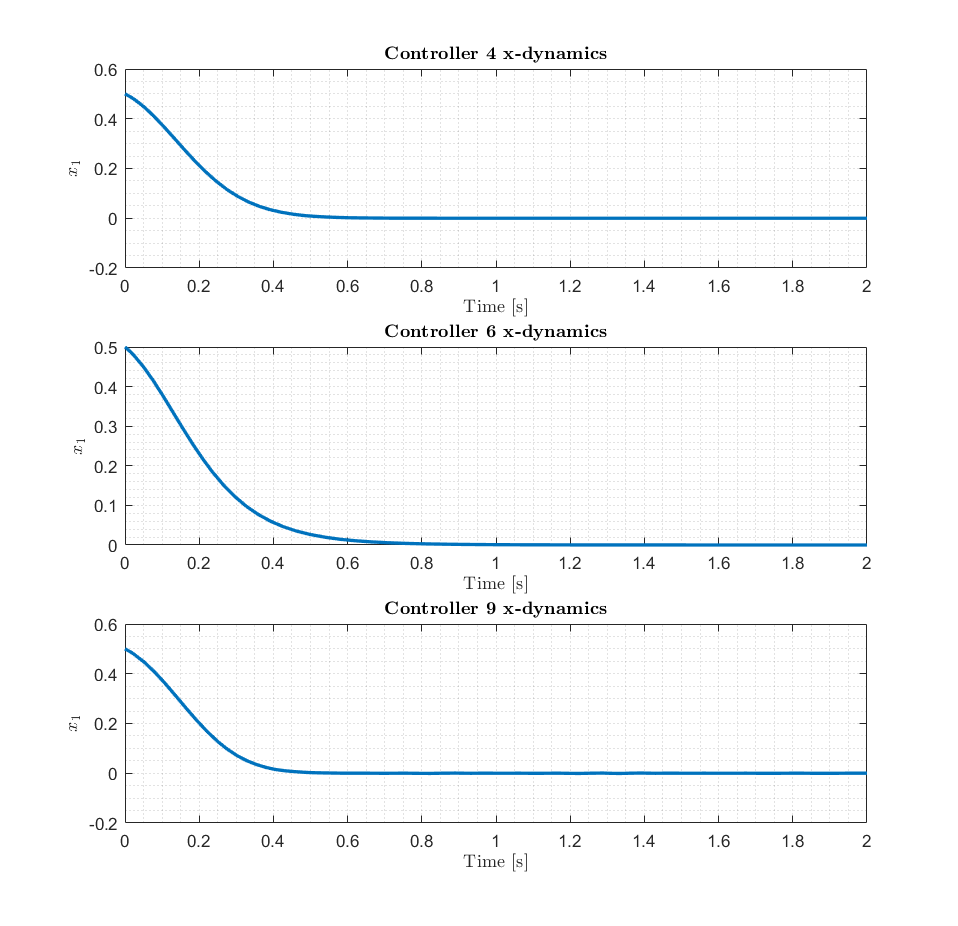
\includegraphics[width=\linewidth]{Figures/sigma_2.png}
  \caption{Response for $\sigma = 2$}
  \label{fig:sigma2}
\end{minipage}
\end{figure}

Because the performance of controller 9 is less dependent on the system parameters this controller is preferred, since this controller is more robust. Furthermore the tuning for this controller turned out to be more easy.


\subsection{Exercise 14}
As can been seen in the subsystem $x_1$ if the value of $x_1$ approaches zero, the time derivative of $x_1$ approaches zero (all terms do depend on $x_1$). Therefore all controllers guarantee that if $x_1(0) > 0$ than $x_1(t) \geq 0$. The same holds for if $x_1(0) < 0$ is negative (The pressure rise is still positive) than $x_1(t) \leq 0$.  Thus the controllers can still be used.


\begin{landscape}
\section{Equation appendix}
\label{Appendix}
\subsection*{Exercise 4}
\begin{equation}
u(z) = \frac{c_{1}\,{z_{1}}^2+c_{2}\,{z_{2}}^2-z_{2}\,z_{3}-c_{3}\,{z_{3}}^2+f_{1}\,z_{3}}{z_{3}}
\label{eq:u_z}
\end{equation}

\begin{dmath}
\dot{V}_3 = -c_{1}\,{z_{1}}^2-c_{2}\,{z_{2}}^2+z_{3}\,z_{2}-f_{1}\,z_{3}+u\,z_{3}
\label{eq:V3d}
\end{dmath}
with:

\begin{dmath}
f_1 = \frac{\partial x_3^v}{\partial z} = \frac{\left(\sigma \,{z_{1}}^4+\sigma \,{z_{1}}^2\,{z_{2}}^2+2\,\sigma \,{z_{1}}^2\,z_{2}-2\,c_{1}\,{z_{1}}^2-2\,c_{2}\,{z_{2}}^2+2\,z_{3}\,z_{2}\right)\,\left(6\,{z_{1}}^2\,{z_{2}}^2+2\,c_{1}\,{z_{1}}^2-2\,c_{2}\,{z_{2}}^2-\sigma \,{z_{1}}^4+6\,{z_{2}}^3+3\,{z_{2}}^4+\sigma \,{z_{1}}^2\,{z_{2}}^2\right)}{4\,{z_{2}}^3}-\frac{\sigma \,{z_{1}}^2\,\left({z_{1}}^2+{z_{2}}^2+2\,z_{2}\right)\,\left(6\,z_{2}-2\,c_{1}+2\,\sigma \,z_{2}+2\,\sigma \,{z_{1}}^2+\sigma \,{z_{2}}^2+6\,{z_{2}}^2\right)}{2\,z_{2}}
\label{eq:f1_report}
\end{dmath}

\subsection*{Exercise 6}%exercise 6
\begin{dmath}
u(z) = \frac{f_{2}\,z_{3}-c_{3}\,{z_{3}}^2-\sigma \,z_{2}\,\left(\frac{3\,z_{2}}{2}+z_{3}-\frac{{\left(z_{2}+1\right)}^3}{2}-c_{1}\,z_{2}-{z_{1}}^2\,\left(3\,z_{2}+3\right)+3\,{z_{1}}^2+\frac{3\,{z_{2}}^2}{2}+\frac{1}{2}\right)+c_{1}\,\sigma \,{z_{1}}^2\,\left({\left(z_{2}+1\right)}^2+{z_{1}}^2-1\right)}{z_{3}}
\label{eq:uz6}
\end{dmath}

\begin{dmath}
\dot{V}_3 = \sigma \,z_{2}\,\left(\frac{3\,z_{2}}{2}+z_{3}-\frac{{\left(z_{2}+1\right)}^3}{2}-c_{1}\,z_{2}-{z_{1}}^2\,\left(3\,z_{2}+3\right)+3\,{z_{1}}^2+\frac{3\,{z_{2}}^2}{2}+\frac{1}{2}\right)-z_{3}\,\left(f_{2}-u\right)-c_{1}\,\sigma \,{z_{1}}^2\,\left({\left(z_{2}+1\right)}^2+{z_{1}}^2-1\right)
\label{eq:V3d6}
\end{dmath}

with:
\begin{equation}
f_2 = \frac{\partial x_3^v}{\partial z} = \frac{\left(c_{1}-3\,z_{2}\right)\,\left(6\,{z_{1}}^2\,z_{2}+{z_{2}}^3+2\,c_{1}\,z_{2}-2\,z_{3}\right)}{2}-3\,\sigma \,{z_{1}}^2\,\left({z_{1}}^2+{z_{2}}^2+2\,z_{2}\right)
\end{equation}


\end{landscape}

\end{document}
